\chapter{Hauptteil}

\section{Architektur der Applikation}

\begin{figure}
	\centering
	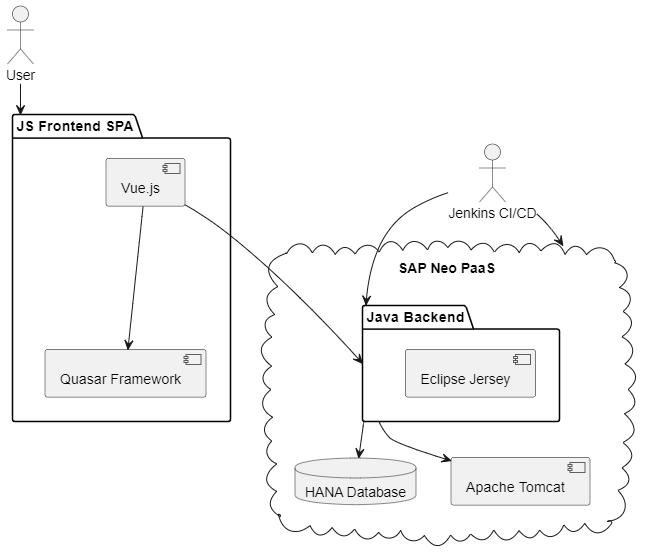
\includegraphics[width=.72\textwidth]{Bilder/architecture.png} 
	\caption{Die Abbildung zeigt die Architektur der Digital Heroes Lernplattform.}
	\label{fig:architecture}
\end{figure} 

Die Architektur der Web-App Digital Heroes mit den verschiedenen verwendeten Technologien
lässt sich in Frontend, Backend und DevOps unterteilen und 
ist in \autoref{fig:architecture} abgebildet. 
Es existieren zwei Instanzen der Architektur: ein Entwicklungs- und ein Produktivsystem. 

\subsubsection*{Frontend:}

Die Frontend-Anwendung der Digital Heroes Web-App ist als Single Page Application (SPA) konzipiert, 
die Vue.js und das Quasar Framework verwendet. 
Vue.js ist ein modernes JavaScript-Framework zum Erstellen von benutzerfreundlichen und reaktiven Webanwendungen.
Quasar ist ein weiteres Framework, das auf Vue.js aufbaut und zusätzliche Funktionen und Komponenten bereitstellt, 
um die Entwicklung von plattformübergreifenden Anwendungen zu erleichtern.
Vue.js nutzt die REST-API des Backends.

\subsubsection*{Backend:}

Das Backend der Web-App besteht aus einer Java-Anwendung, die Eclipse Jersey und Apache Tomcat verwendet. 
Eclipse Jersey ist eine Implementierung der JAX-RS-Spezifikation 
und ermöglicht die einfache Entwicklung von RESTful Web Services für Servlet Container. 
Apache Tomcat ist ein Servlet-Container, der als Webserver zum Bereitstellen von Java-Anwendungen dient
und das Java-Backend hostet.
Als Datenbank kommt die HANA-Datenbank zum Einsatz, die eine high-performance, in-memory relationale Datenbank ist 
und von SAP entwickelt wird. 
Das Java-Backend nutzt das Eclipse-Framework und die HANA-Datenbank um eine REST-API für das 
Vue.js-Frontend bereitzustellen. 

\subsubsection*{DevOps:}

Im Bereich der DevOps-Infrastruktur kommt Jenkins zum Einsatz, 
eine Open-Source-Automatisierungssoftware, 
die zur Implementierung von Continuous Integration und Continuous Deployment (CI/CD) verwendet wird. 
Jenkins ermöglicht die Automatisierung von Build- und Testprozessen sowie die Bereitstellung 
der Anwendung in einer kontrollierten und konsistenten Weise. 
Die Web-App wird auf der SAP Neo Platform-as-a-Service (PaaS) Cloud-Plattform gehostet, 
die eine skalierbare und einfach zu verwaltende Umgebung für die Bereitstellung 
und den Betrieb der Anwendung bietet.
Wird auf den Main-Branch des verwendeten Github-Respositories gepusht, bzw. eine Pull-Request gemerged,
startet Jenkins den CI/CD-Prozess und testet und deployed das neue Backend/Frontend auf der Entwicklungsinstanz. 
Änderungen im Frontend werden zudem direkt auf dem Produktivsystem deployed. 
Für Änderungen des Backends im Produktivsystem kann in SAP Neo ein neuer Release erzeugt werden, 
bei dem das Java-Backend der Entwicklungsinstanz auf das Produktivsystem kopiert wird. 


\section{Ist-Situation und warum die problematisch ist}

Das Entwickler-Team ist auf Deutschland und Australien aufgeteilt, 
was zu Kommunikationsschwierigkeiten und unterschiedlichen Arbeitszeiten führen kann. 
Dies erschwert die Zusammenarbeit und kann die Qualität der Software und die Effizienz 
der Entwicklungsprozesse beeinträchtigen.

Es gibt keine fest vorgegebenen Release-Zyklen; Releases finden nur statt, 
wenn ein neues Feature fertig ist. Dies kann zu unvorhersehbaren und unregelmäßigen Updates führen,
wodurch die Planung und das Management des Projekts schwieriger werden.

Releases werden oft freitags durch das australische Team durchgeführt. 
Dies kann problematisch sein, weil das Team in Deutschland möglicherweise nicht verfügbar ist, 
um eventuell auftretende Probleme sofort zu beheben, was zu längeren Ausfallzeiten führen kann.

Es gibt keinerlei automatisierte Tests. Dies bedeutet, 
dass die Qualität der Software nicht kontinuierlich überprüft wird, 
wodurch Fehler erst spät oder gar nicht entdeckt werden. Dies erhöht das Risiko, 
dass Fehler in die Produktion gelangen, was zu einer schlechteren Benutzererfahrung führt.

Viele Bugs gelangen in die Produktionsumgebung, wodurch oft Hot-Fixes notwendig sind. Dies zeigt, 
dass der Entwicklungsprozess und die Qualitätssicherung unzureichend sind und die Softwarequalität leidet.

Der CI/CD-Prozess für das Deployment auf der Entwicklungsinstanz dauert 15 Minuten. 
Das ist eine lange Wartezeit, die den Entwicklungsprozess verlangsamt und zu einer geringeren Produktivität führt.

Das Backend kann nicht auf dem lokalen Rechner gestartet werden, 
da die HANA-Datenbank nicht lokal gehostet werden kann und kein Mock existiert. 
Dies erschwert die lokale Entwicklung und das Testen, 
was die Effizienz der Entwickler beeinträchtigt und die Qualität der Software gefährdet.

Die Codequalität ist in einem schrecklichen Zustand: Viele duplikative Code-Stücke, 
wenig Struktur und keine Aufteilung der Architektur in Schichten. 
Es wird immer gegen Implementierungen programmiert, anstatt gegen Abstraktionen. 
Dies führt zu einer schlechteren Wartbarkeit, 
erhöht die Fehleranfälligkeit und erschwert die Einarbeitung neuer Teammitglieder.

Der Code ist oft unleserlich, zum Beispiel durch 40-50 Zeilen lange, 
verschachtelte SQL-Statements, die viel Code-Duplikate enthalten. 
Dies führt zu einer schlechteren Wartbarkeit und macht es schwieriger, 
Fehler zu erkennen und zu beheben.

Es gibt keine Code-Reviews, was bedeutet, dass keine systematische Überprüfung der Codequalität 
stattfindet. Dies erhöht die Wahrscheinlichkeit von Fehlern und mindert die Qualität der Software.

Obwohl ein Kanban-Board mit Tasks und Prioritäten verwendet wird, 
gibt es kein Sprint-Planning und kein Sprint-Review. 
Dies führt zu einer schlechteren Planung und Kontrolle der Arbeit 
und beeinträchtigt die Effizienz des Entwicklungsprozesses.

Die Scrum-Meetings finden zweimal pro Woche statt, 
aber mit der ganzen Abteilung (nicht nur Entwickler, sondern auch Designer, Manager, Content-Moderatoren usw.). 
Dadurch werden diese Meetings sehr ineffizient, 
da nicht alle Teilnehmer direkt am Entwicklungsprozess beteiligt sind. 
Dies führt zu einer schlechteren Kommunikation und Koordination innerhalb des Entwicklerteams 
und beeinträchtigt die Effizienz des Entwicklungsprozesses.

Insgesamt sind die identifizierten Probleme im Bereich der Software-Qualitäts-Management 
und Entwicklungsprozesse ein erhebliches Hindernis für die Erreichung einer 
hohen Softwarequalität und einer effizienten Arbeitsweise. Um die Situation zu verbessern, 
müssen die genannten Probleme adressiert und Lösungen gefunden werden, 
die zu einer besseren Organisation, Kommunikation und Qualitätssicherung führen.